\documentclass[12pt]{article}
\usepackage[margin=1in]{geometry}
\usepackage{amsmath,amssymb,amsfonts}
\usepackage{graphicx}
\usepackage{booktabs}
\usepackage{array}
\usepackage{float}
\usepackage{caption}
\usepackage{hyperref}

\title{Control of an Inverted Pendulum Using LQR and Model Predictive Control}
\author{Your Name \\ Course / Section}
\date{\today}

\begin{document}

\maketitle

\begin{abstract}
This report presents the modeling and control of a linearized cart-pole inverted pendulum system using two state-space control strategies: Linear Quadratic Regulator (LQR) and Model Predictive Control (MPC). The work extends a baseline LQR design with two MPC implementations developed in MATLAB: a condensed prediction-matrix formulation and a recursive formulation with terminal equality constraints. The objective is to regulate the pendulum angle near the upright equilibrium while controlling cart motion and keeping the control effort bounded. Simulation scripts show that the controller behavior is highly sensitive to the MPC horizon, weighting matrices, and terminal constraints. In particular, the recursive MPC formulation gives a more structured tracking setup, while the shorter-horizon condensed MPC case can become unstable.
\end{abstract}

\section{Introduction}
The inverted pendulum is a standard benchmark for evaluating feedback control algorithms because it is inherently unstable, nonlinear, and underactuated. A controller must stabilize the pendulum angle while also managing the cart position and the applied force. These competing objectives make the system a useful case study for optimal control.

This project considers a linearized cart-pole model and compares LQR with MPC. The LQR controller provides a compact full-state feedback law based on quadratic performance criteria. MPC, in contrast, explicitly predicts future outputs over a finite horizon and handles input constraints through online optimization. The goal of this report is to document the mathematical model, summarize the controller designs implemented in MATLAB, and discuss the observed simulation behavior.

\section{System Model}
\subsection{Physical Parameters}
The system parameters used throughout the MATLAB scripts are
\begin{align*}
M &= 0.5~\text{kg}, &
m &= 0.2~\text{kg}, &
b &= 0.1~\text{N}\cdot\text{s/m}, \\
I &= 0.006~\text{kg}\cdot\text{m}^2, &
g &= 9.8~\text{or}~9.81~\text{m/s}^2, &
l &= 0.3~\text{m}.
\end{align*}

The state vector is chosen as
\[
x = \begin{bmatrix}
x & \dot{x} & \phi & \dot{\phi}
\end{bmatrix}^T,
\]
where $x$ is the cart position and $\phi$ is the pendulum angle relative to the upright equilibrium.

\subsection{Linearized State-Space Model}
Using the standard small-angle linearization about the upright position, the continuous-time dynamics are
\[
\dot{x}(t) = A x(t) + B u(t), \qquad y(t) = Cx(t) + Du(t),
\]
with
\[
p = I(M+m)+Mm l^2,
\]
and
\[
A =
\begin{bmatrix}
0 & 1 & 0 & 0 \\
0 & -\dfrac{(I+ml^2)b}{p} & \dfrac{m^2 g l^2}{p} & 0 \\
0 & 0 & 0 & 1 \\
0 & -\dfrac{mlb}{p} & \dfrac{mgl(M+m)}{p} & 0
\end{bmatrix},
\qquad
B =
\begin{bmatrix}
0 \\
\dfrac{I+ml^2}{p} \\
0 \\
\dfrac{ml}{p}
\end{bmatrix}.
\]

The measured outputs are cart position and pendulum angle:
\[
C =
\begin{bmatrix}
1 & 0 & 0 & 0 \\
0 & 0 & 1 & 0
\end{bmatrix},
\qquad
D =
\begin{bmatrix}
0 \\
0
\end{bmatrix}.
\]

The MATLAB code also includes the transfer-function representation for the cart position and pendulum angle channels, confirming consistency between the transfer-function and state-space descriptions.

\section{LQR Controller Design}
\subsection{Design Setup}
The LQR controller is implemented in \texttt{IP\_LQR.m}. The script first checks the system poles and controllability, then computes a state-feedback gain of the form
\[
u(t) = -Kx(t).
\]

The quadratic cost is
\[
J = \int_0^\infty \left(x^TQx + u^TRu\right)\,dt,
\]
with weighting matrices selected in the MATLAB script as
\[
Q = C^T C, \qquad Q_{11}=5000, \qquad Q_{33}=100, \qquad R=1.
\]

This choice places a strong penalty on cart position error and a moderate penalty on pendulum angle deviation. The resulting controller is then simulated for a reference input of $0.2$~m.

\subsection{Interpretation}
The LQR design offers a simple full-state feedback solution with low implementation complexity. Since the gain is computed offline, the online control law is computationally inexpensive. However, standard LQR does not directly enforce actuator constraints. In this project, it serves as a useful baseline against which the MPC controllers can be compared.

\section{MPC Design}
Two MPC formulations were implemented: a condensed prediction-matrix formulation in \texttt{IP\_MPC.m} and a recursive formulation in \texttt{IP\_MPC\_RECURSIVE.m}. Both use the discretized linear model with sampling time
\[
T_s = 0.01~\text{s}.
\]

\subsection{Discrete-Time Model}
The continuous-time system is discretized in MATLAB using \texttt{c2d}, producing
\[
x_{k+1} = A_d x_k + B_d u_k, \qquad y_k = C_d x_k.
\]

This discrete-time model is used for prediction over a finite horizon.

\subsection{Condensed MPC Formulation}
In \texttt{IP\_MPC.m}, the prediction horizon is chosen as
\[
N = 5.
\]
The output and input penalties are
\[
Q_y = \mathrm{diag}(50,50), \qquad R_u = 0.01,
\]
which are lifted over the horizon using Kronecker products:
\[
Q = I_N \otimes Q_y, \qquad R = I_N \otimes R_u.
\]

The future outputs are written in compact form as
\[
Y = \Gamma x_k + \Theta U,
\]
where $U$ is the stacked control vector over the horizon. The optimization problem solved at each sampling instant is
\begin{align*}
\min_U \quad & (Y-R_f)^TQ(Y-R_f) + U^TRU \\
\text{subject to} \quad & u_{\min} \le U \le u_{\max},
\end{align*}
with
\[
u_{\min}=-10, \qquad u_{\max}=10.
\]
In the current script, the reference vector is initialized as
\[
R_f = 0,
\]
so the controller acts as a regulator about the origin.

The initial condition used in the simulation is
\[
x_0 =
\begin{bmatrix}
0.05 & 0 & 0.15 & 0
\end{bmatrix}^T.
\]

\subsection{Recursive MPC Formulation}
In \texttt{IP\_MPC\_RECURSIVE.m}, the optimization is posed directly in terms of predicted states and inputs:
\[
\{x_{k|k},x_{k+1|k},\dots,x_{k+N|k}\}, \qquad \{u_{k|k},\dots,u_{k+N-1|k}\}.
\]

The prediction horizon is increased to
\[
N = 30,
\]
and the script comments note that infeasibility occurs for $N < 30$ because of the terminal constraint.

The stage cost is
\[
\ell(x_{i|k},u_{i|k}) = (y_{i|k}-r)^TQ(y_{i|k}-r) + u_{i|k}^TRu_{i|k},
\]
with
\[
Q = \mathrm{diag}(200,200), \qquad R = 0.01,
\qquad
r = \begin{bmatrix} 0.2 \\ 0 \end{bmatrix}.
\]

The optimization problem is
\begin{align*}
\min_{\{x_{i|k},u_{i|k}\}} \quad &
\sum_{i=1}^{N}
\left[
(y_{i|k}-r)^TQ(y_{i|k}-r) + u_{i|k}^TRu_{i|k}
\right] \\
\text{subject to} \quad &
x_{i+1|k} = A_d x_{i|k} + B_d u_{i|k}, \\
& u_{\min} \le u_{i|k} \le u_{\max}, \\
& x_{0|k} = x_k, \\
& x_{N|k} = x_{\mathrm{ref}},
\end{align*}
where
\[
x_{\mathrm{ref}} =
\begin{bmatrix}
0.2 & 0 & 0 & 0
\end{bmatrix}^T.
\]

This terminal equality constraint makes the optimization more restrictive but gives a clear target at the end of the horizon. Only the first control move is applied at each step, and the problem is solved again at the next sample, following the standard receding-horizon principle.

\section{Simulation Setup}
Both MPC scripts simulate the system for
\[
T_{\mathrm{sim}} = 500
\]
steps, corresponding to a total time of
\[
500 \times 0.01 = 5~\text{s}.
\]

The LQR script also uses a $0.01$~s simulation grid over $5$~s. All controllers plot the cart position, pendulum angle, and control force. The optimization problems in the MPC implementations are solved in YALMIP using \texttt{quadprog}.

\section{Results and Discussion}
\subsection{LQR}
The LQR controller provides a conventional stabilizing solution for the linearized system. Because the controller uses full-state feedback and quadratic penalties, it is expected to balance cart-position tracking with pendulum-angle suppression while maintaining moderate control effort. The method is computationally efficient and suitable when explicit constraints are not a primary concern.

\subsection{Condensed MPC}
The condensed MPC controller includes actuator bounds but uses a short horizon and no terminal cost or terminal constraint. Based on the provided simulation image, the pendulum-angle response can diverge significantly while the input saturates at the lower bound of $-10$~N. This suggests that the short-horizon setup is not sufficient to guarantee practical closed-loop stability for the chosen weights and initial condition.

\begin{figure}[H]
    \centering
    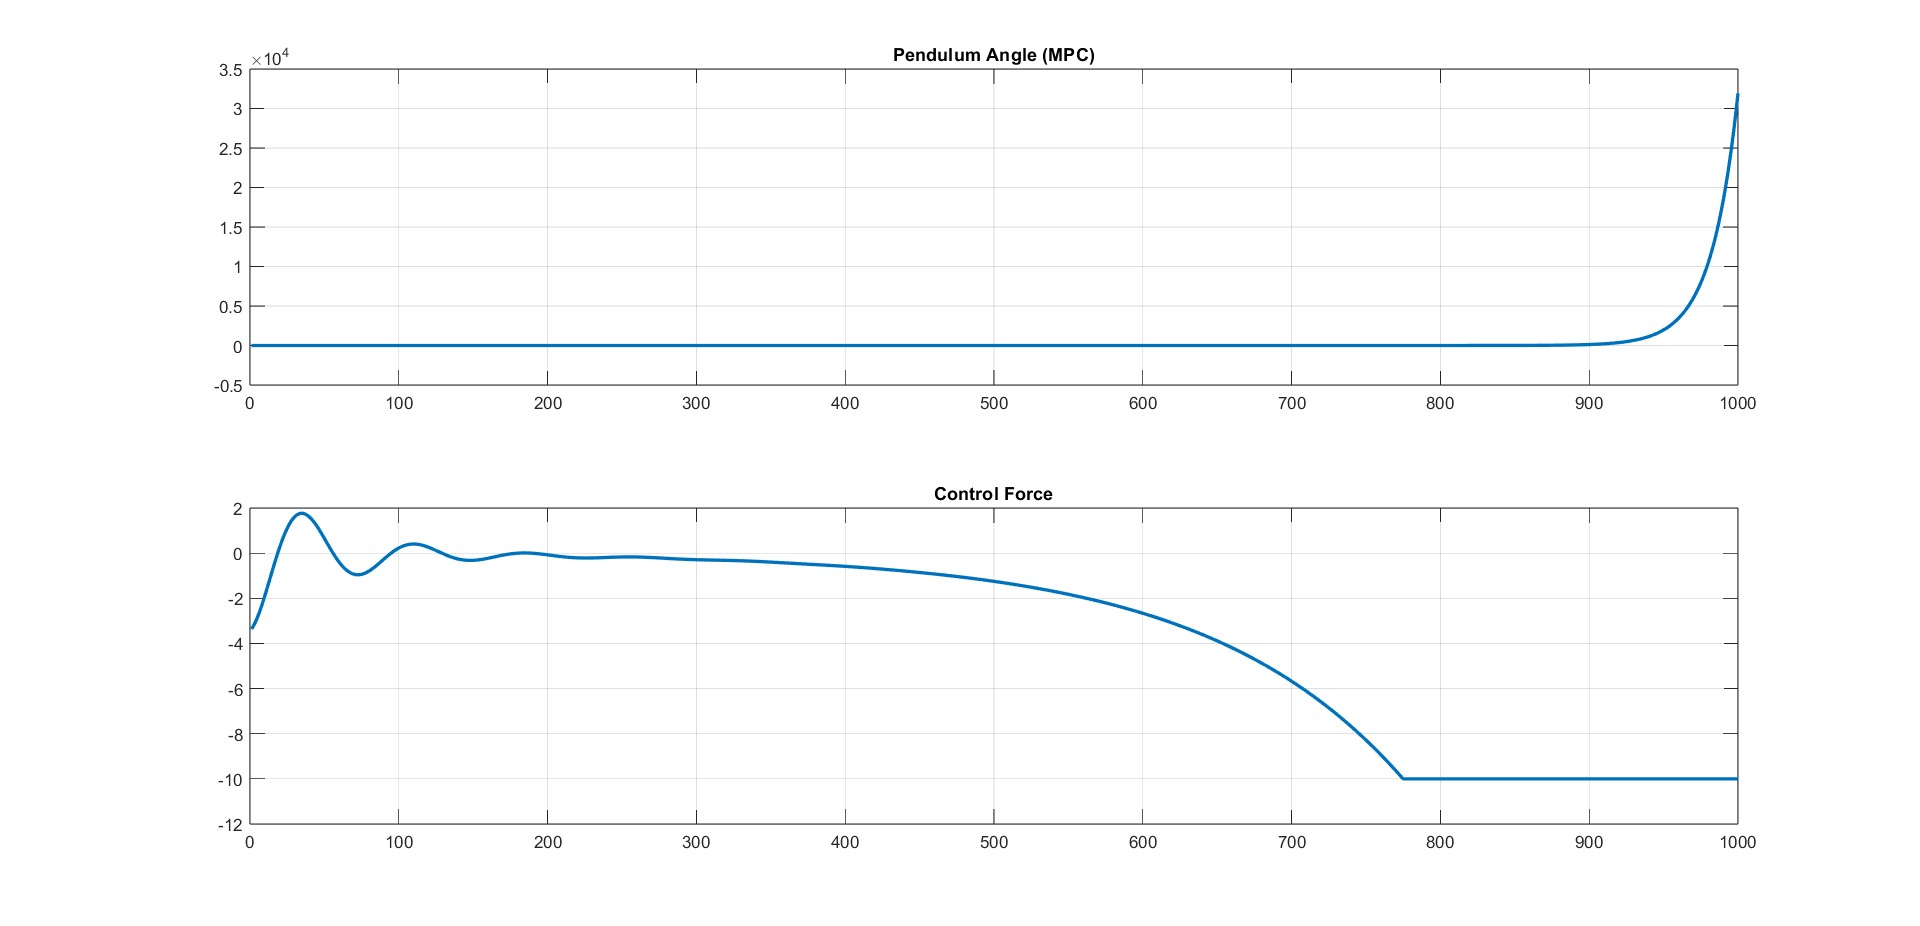
\includegraphics[width=0.95\textwidth]{q20_200.jpg}
    \caption{Example MPC response showing pendulum-angle growth and input saturation in the constrained condensed formulation.}
    \label{fig:mpc_unstable}
\end{figure}

Several factors contribute to this behavior:
\begin{itemize}
    \item the horizon $N=5$ is short for an unstable plant,
    \item the reference is set to zero regulation only,
    \item the formulation does not include a terminal cost or terminal invariant set,
    \item actuator saturation limits the controller's authority once the state grows.
\end{itemize}

\subsection{Recursive MPC}
The recursive MPC design is more structured. It uses a longer horizon, stronger output weighting, and a terminal equality constraint that forces the predicted state to end at the desired equilibrium. The code comments indicate that this formulation becomes infeasible for shorter horizons, which is consistent with the restrictive nature of exact terminal constraints.

Compared with the condensed formulation, this controller is better aligned with reference tracking because it explicitly penalizes deviation from
\[
r = \begin{bmatrix}0.2 & 0\end{bmatrix}^T
\]
and drives the full predicted terminal state to
\[
x_{\mathrm{ref}} =
\begin{bmatrix}
0.2 & 0 & 0 & 0
\end{bmatrix}^T.
\]
The tradeoff is increased online computational effort and possible feasibility issues if the horizon is too short or the constraints are too restrictive.

\section{Comparison of LQR and MPC}
The main differences between the controller designs in this project are summarized in Table~\ref{tab:comparison}.

\begin{table}[H]
\centering
\caption{Comparison of control approaches}
\label{tab:comparison}
\begin{tabular}{>{\raggedright\arraybackslash}p{2.4cm} >{\raggedright\arraybackslash}p{4.8cm} >{\raggedright\arraybackslash}p{4.8cm}}
\toprule
Method & Advantages & Limitations \\
\midrule
LQR & Simple full-state feedback, low online computation, good baseline stabilizer & Does not explicitly enforce input constraints, less flexible for tracking and constrained operation \\
Condensed MPC & Explicitly handles input bounds, optimization-based design & Short horizon can produce poor behavior on unstable plants, no terminal ingredients in current script \\
Recursive MPC & Natural tracking formulation, direct state/input constraints, terminal target included & Higher computational cost, terminal equality can cause infeasibility for short horizons \\
\bottomrule
\end{tabular}
\end{table}

\section{Conclusion}
This project studied the control of an inverted pendulum using LQR and two MPC implementations. The LQR controller provides an efficient unconstrained baseline, while MPC offers the ability to enforce actuator limits and shape future behavior through optimization. The simulation setup also shows that MPC performance depends strongly on formulation details. A short-horizon condensed MPC can become unstable for the chosen tuning, whereas the recursive MPC with terminal constraints gives a more principled tracking design at the cost of increased complexity and feasibility sensitivity.

Future improvements would include adding a terminal cost or terminal set to the condensed MPC formulation, tuning the prediction horizon and weights more systematically, and comparing all controllers using common initial conditions and quantitative performance metrics such as settling time, overshoot, and control energy.

\section*{Appendix: MATLAB Files Used}
The report is based on the following scripts in the project folder:
\begin{itemize}
    \item \texttt{IP\_LQR.m}
    \item \texttt{IP\_MPC.m}
    \item \texttt{IP\_MPC\_RECURSIVE.m}
    \item \texttt{inverted\_pendulum\_ss.m}
    \item \texttt{Inverted\_pendulum\_tf.m}
    \item \texttt{IP\_PID.m}
\end{itemize}

\end{document}
